\chapter{Review of Related Literature}
\section{PCOS}

PCOS is a multifaceted endocrine, metabolic, and reproductive disorder affecting a significant number of reproductive-aged women globally. Characteristic manifestations include hyperandrogenism, oligo-anovulation, polycystic ovarian morphology, and insulin resistance via preferential abdominal fat accumulation (Dumesic et al., 2022). 

Four phenotypes have been identified which group the multifaceted symptoms of the disorder when observed via ultrasound (See \ref{tab:Phenotypes}) (Khan et al., 2017). Phenotypes A and B are the classic representation of PCOS and are characterized by oligoanovulation and hyperandrogenism, with type A further possessing multiple polycystic ovaries. Given that the two differ solely in terms of ovarian morphology, endocrine or metabolic differences do not exist. Phenotype C (ovulatory PCOS) is characterized by polycystic ovaries with the occurrence of routine menses and hyperandrogenism. Lastly, phenotype D (Nonhyperandrogenic PCOS) is marked by polycystic ovaries, oligoanovulation, and the lack of hyperandrogenism. The NIH diagnostic criteria recognize phenotypes A and B, the Rotterdam criteria accept all four phenotypic groups, and the AES classification takes into account the first three phenotypic classes only (Lujan et al., 2008; Khan et al., 2017). Proper classification of the phenotypes is crucial for the correct diagnosis of the disease and implementation of suitable treatment strategies. 

% \usepackage{tabularray}
\begin{table}
    \centering
    \caption{PCOS Phenotypes and Corresponding Manifestations}
    \label{tab:Phenotypes}
\begin{tblr}{
  row{odd} = {c},
  row{2} = {c},
  row{4} = {c},
  cell{2}{2} = {r=2}{},
  hline{1-2,6} = {-}{},
}
\textbf{Phenotype} & \textbf{Type}       & \textbf{Manifestations}                                \\
A                  & Classical           & Hyperandrogenism, oligoanovulation, polycystic ovaries \\
B                  &                     & Hyperandrogenism and oligoanovulaiton                  \\
C                  & Ovulatory           & Hyperandrogenism and polycystic ovaries                \\
D                  & Nonhyperandrogenic~ & Oligoanovulation and polycystic ovaries                \\
                   &                     &                                                        
\end{tblr}
\end{table}

\section{Multifaceted Pathology of PCOS}

PCOS patients may experience adverse manifestations due to the presence of excess male sex hormones such as hirsutism, androgenic alopecia, and acne–commonly known as hyperandrogenism (Wang \& Li, 2023). The CYP11A1 gene mainly functions in the catalysis of cholesterol to pregnenolone which is necessary in steroidogenesis or the synthesis of sex hormones. A promoter pentanucleotide repeat (tttta)n polymorphism in this gene is often associated with elevated androgen levels and is considered a risk molecular marker for PCOS. A case-control study that evaluated the PCOS susceptibility of CYP11A1 polymorphism from extracted, amplified, and genotyped DNA of 267 PCOS patients and 275 controls from South India found that alleles with repeats above 8 exhibited a three-fold risk for PCOS susceptibility as compared to the controls (Reddy et al., 2014). 

Another gene involved in steroidogenesis is CYP17A1 which converts pregnenolone and progesterone into 17-hydroxypregnenolone and 17-hydroxyprogesterone and inverts these steroids into dehydroepiandrosterone (DHEA) and $\Delta$4-Androstendione ($\Delta$4A), which is catalyzed by the P450c17 enzyme (Panda et al., 2016). Polymorphism in this gene was found to increase body weight, IR, and excessive lipid in a study conducted on the Chilean population (Ajmal et al., 2019). Moreover, the enzymatic activity of P450c17 was observed to increase the abundance of ovary theca cells in PCOS women (Panda et al., 2016).

Abnormal levels of gonadotropin secretion are another manifestation of PCOS that is influenced by an elevated level of luteinizing hormones (LH) and low levels of follicle-stimulating hormone (FSH). Decreased levels of FSH increase the risk of infertility due to the failure of the follicle to mature and consequently release eggs. Follicular cysts emerge in follicles that fail to ovulate and are characterized by an increased abundance of follicular fluid and the absence of an oocyte (Ndefo et al., 2013). 

Metabolic aberrations due to excess androgen are also notable pathologic factors of PCOS. Specifically, type 2 diabetes or glucose intolerance has been shown to have higher occurrences in PCOS women despite the absence of obesity (Christakou \& Diamanti-Kandarakis, 2008). However, more complex metabolic phenotypes may arise in the presence of obesity, which accounts for approximately 50\% of PCOS women, due to the added interactions with metabolic abnormalities. Ehrmann et al. (1999) found that 45\% of 122 women with clinical and hormonal evidence of PCOS showed abnormal levels of glucose tolerance. Additionally, evidence has shown the increased pathogenesis of type 2 diabetes mellitus in obese individuals due to the stimulation of IR (Wondmkun, 2020).

\section{Insulin Resistance and PCOS}
IR has been identified as the predominant manifestation among women diagnosed with PCOS due to the aberrant functioning of one or more elements of the insulin transduction pathway (Zhao et al., 2023). Within the context of PCOS, the dysfunction of this molecular process effectively decreases tissue sensitivity to insulin, resulting in impaired insulin-stimulated glucose transport and inhibited lipolysis in adipose tissue; reduced insulin-mediated glucose processing in skeletal muscle; impaired gluconeogenesis suppression but stimulated fatty acid synthesis in liver tissue; and, androgen-dependent anovulation in the ovaries and uterus (Hardy et al., 2012; Zhao et al., 2023).

Under physiologically normal conditions, insulin binds to its receptor, activating a tyrosine kinase. This leads to further autophosphorylation of the insulin receptor beta subunit, which in turn phosphorylates insulin receptor substrates (IRS) that serve as docking sites for phosphoinositide 3-kinases (PI3K). Activation of PI3K directly enables the translocation GLUT-4 transporters to the cell surface which facilitates insulin-dependent glucose uptake by cells (See \ref{fig:InsulinPath}). Additionally, activated PI3K leads to the phosphorylation of protein kinase B (PKB or Akt), which subsequently phosphorylates glycogen synthase kinase-3 (GSK3), effectively inactivating it. Due to GSK3 inactivation, glycogen synthase is activated to catalyze glycogenesis (Diamanti-Kandarakis \& Papavassiliou, 2006). 

\begin{figure} 
            \centering
            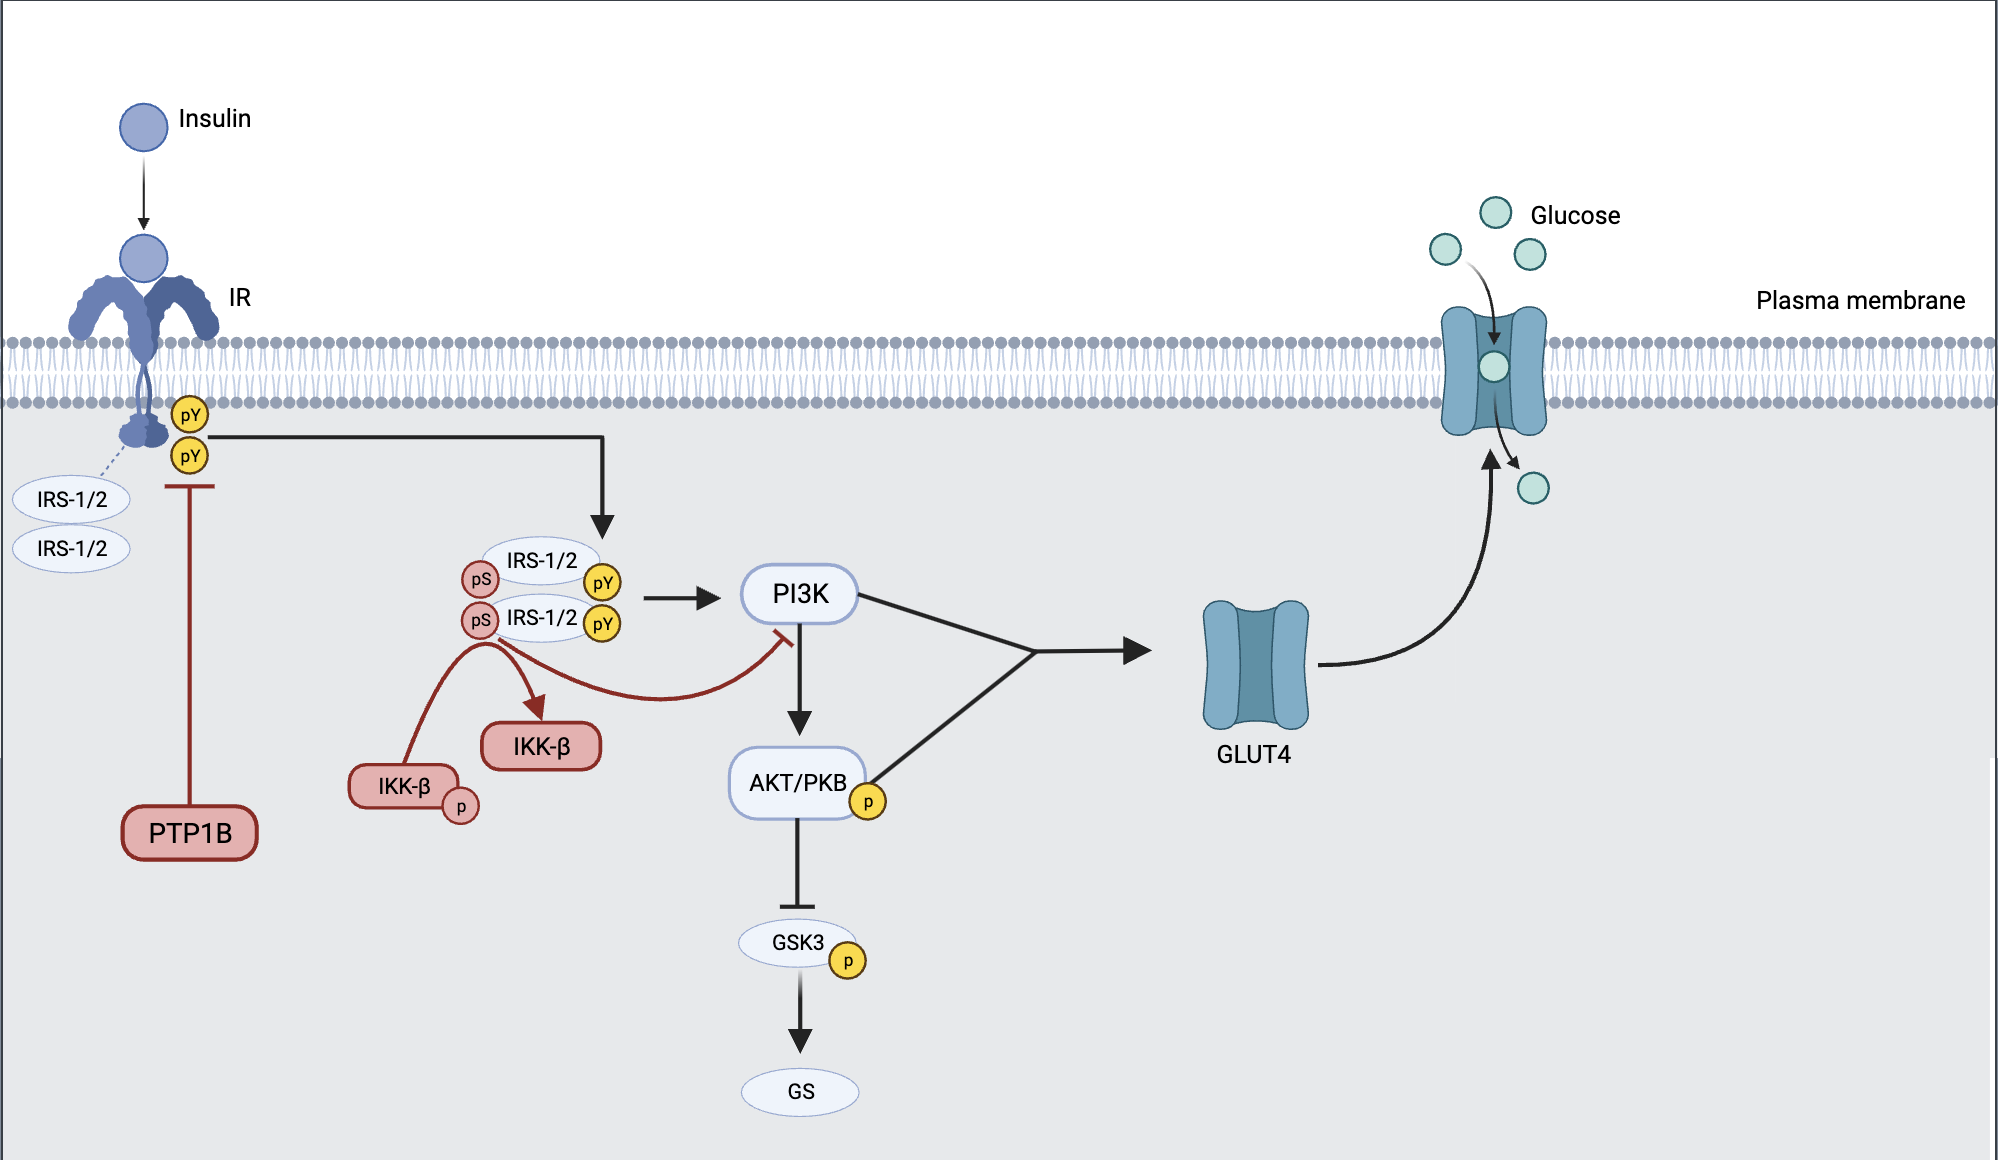
\includegraphics[width=1\linewidth]{Images/pathway.png}
            \caption{Insulin Signal Transduction Pathway}
            \label{fig:InsulinPath}
        \end{figure}

\subsection{PCOS Aberrant Insulin Pathway}
However, women with PCOS are unable to perform this standard mechanism likely due to multiple irregularities. In the insulin signal transduction pathway of PCOS women, it has been suggested that increased serine phosphorylation and decreased tyrosine phosphorylation of insulin receptors and insulin receptor substrate proteins (IRS) can terminate insulin action (Diamanti-Kandarakis \& Dunaif, 2012). Thus, despite the unaltered affinity of insulin to its receptor, insulin dysfunction may still result due to post-binding defects in insulin signal transduction. 

To illustrate, a study found that 50\% of PCOS-cultured skin fibroblasts presented decreased insulin receptor autophosphorylation due to decreased insulin-dependent tyrosine phosphorylation and increased insulin-independent receptor serine phosphorylation. The latter is known to inhibit receptor tyrosine kinase activity, thereby terminating the insulin-signaling pathway in its early steps. Furthermore, this abnormality has also been observed in insulin receptors isolated from classic insulin target tissues, specifically skeletal muscle. This trend of increased insulin-independent serine phosphorylation seems to be unique to PCOS as this tendency is not observed in other insulin disorders like non-insulin-dependent diabetes mellitus. 

On the other hand, the other 50\% of skin fibroblasts from PCOS women did not exhibit the abnormality in insulin receptor phosphorylation. However, there was a decrease in muscle PI3K activation during insulin infusion, and thus reduced translocation of GLUT-4 to the cell surface. Additionally, a recent study found elevated phosphorylation residues on IRS-1 and IRS-2, resulting in lower insulin-mediated IRS-1-related PI3K activation due to targeted IRS-1 destruction. In conjunction with these findings, other studies of skeletal muscle have demonstrated reduced phosphorylation of PKB and the PKB substrate. As such, it has been hypothesized that a defect downstream of insulin receptor signaling, namely, phosphorylation of IRS-1 or activation of PI3K is responsible (Dunaif et al. 1995 as cited in Dunaif, 1997).

\subsection{Protein tyrosine phosphatase 1B in PCOS}
Human protein tyrosine phosphatase 1B (PTP1B, PDB ID: \href{https://www.rcsb.org/structure/4I8N}{4I8N}) is a 435 amino acid-long, 49 kDa peripheral membrane protein of the endoplasmic reticulum encoded by the PTPN1 gene. It is an asymmetric monomer of the non-receptor protein tyrosine phosphatases (non-receptor class I subfamily), composed of an N-terminal catalytic domain (1-300), a regulatory domain (301-400), and a C-terminal domain (400-435). Specifically, binding sites include residue 181, 215-221, and 262, while the active site is marked on a cysteine residue at position 215 (Bateman et al., 2022; Liu et al., 2022)

The N-terminal catalytic domain is composed of eight $\alpha$-helices and twelve $\beta$-strands (see \ref{fig:4i8n}).  It is regulated by post-translational modifications such as the phosphorylation of serine and tyrosine residues and the oxidation of the catalytic cysteine (Cys215). For instance, phosphorylation of Ser50 decreases PTP1B activity, thus hindering PTP1B-mediated dephosphorylation of the insulin receptor. Conversely, phosphorylation of Tyr66 in response to insulin stimulation leads to the negative regulation of the insulin pathway. The catalytic cysteine, however, was identified to modulate the degree and duration of phosphotyrosine-dependent signaling wherein its oxidation would terminate PTP1B activity transiently or permanently depending on its oxidized form (Liu et al., 2022).  

    \begin{figure} 
        \centering
        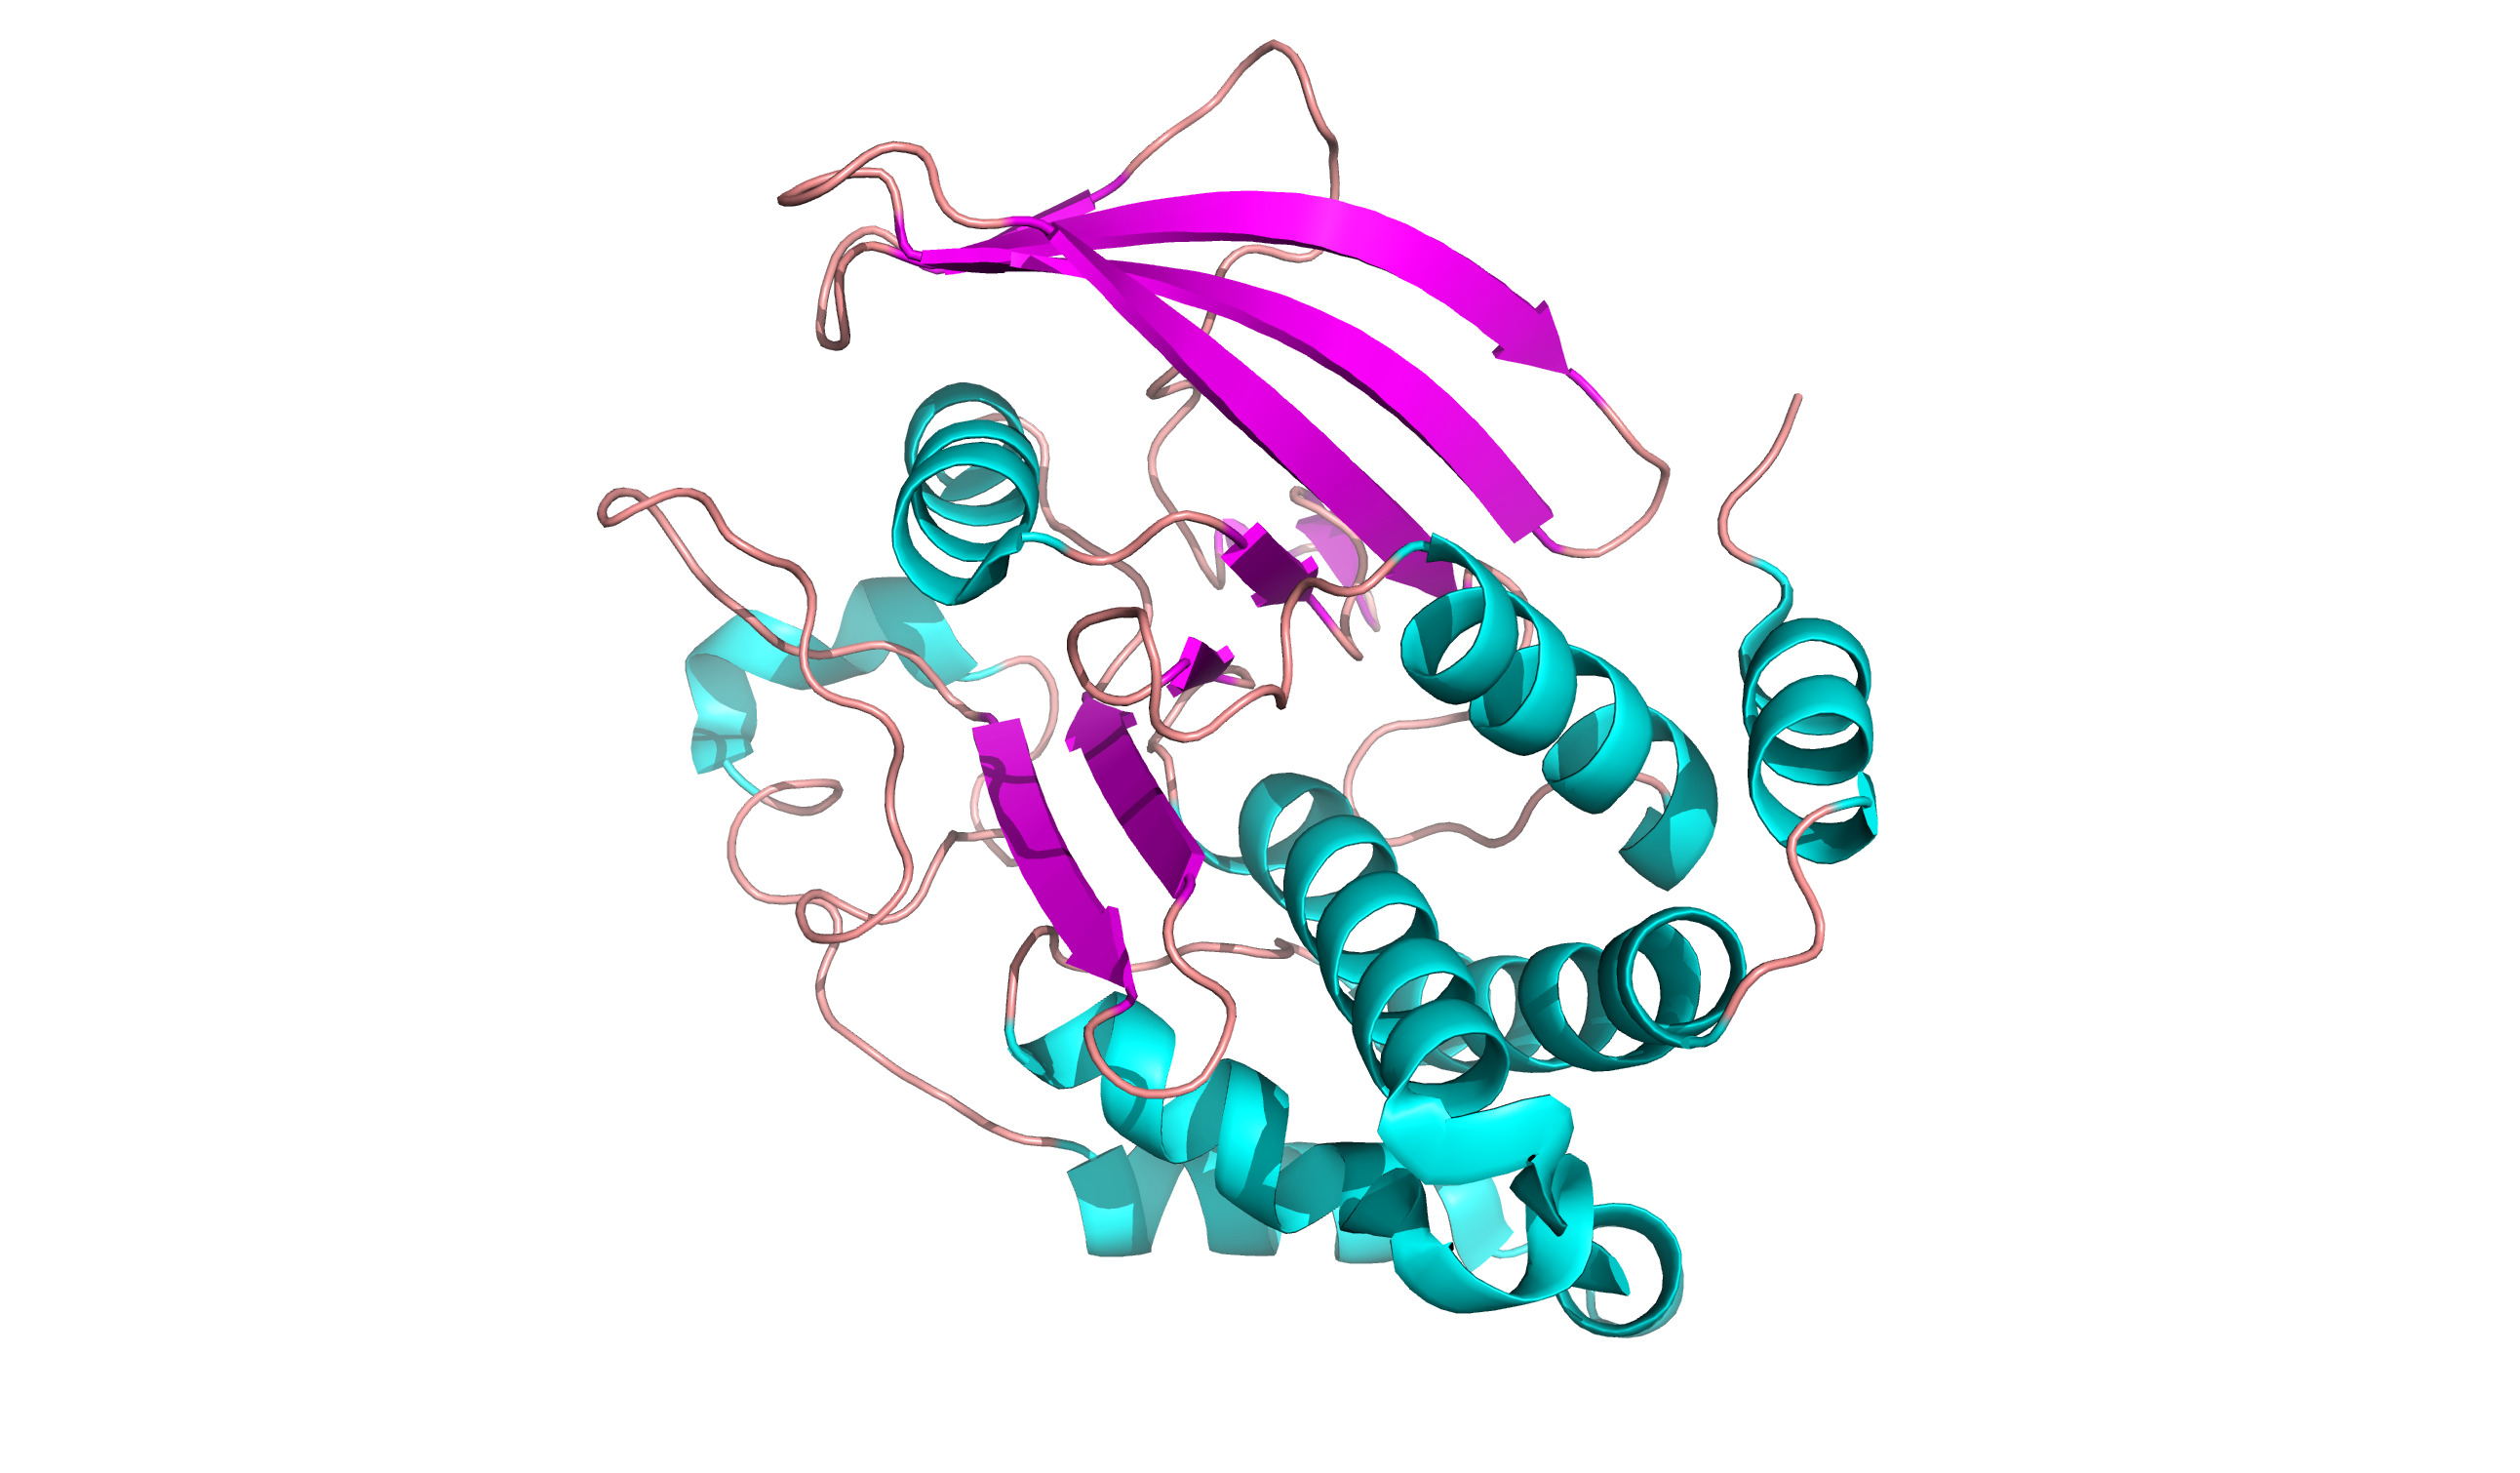
\includegraphics[width=1\linewidth]{Images/4i8n_ss.png}
        \caption{X-ray crystallographic structure of PTP1B}
        \label{fig:4i8n}
    \end{figure}

The regulatory domain is proline-rich and functions as an interaction site for Src homology 3 domain-containing proteins. Substituting crucial proline residues inhibits PTP1B from binding to and activating Src, but it does not impact its dephosphorylating function on insulin receptors (Liu et al., 2022). With this, it is crucial to signal transduction mechanisms of insulin, leptin, growth hormone, and endoplasmic reticulum stress (Delibegović \& Mody, 2013). 

Within the context of insulin resistance specifically, PTP1B is a negative regulator of insulin signaling and normally catalyzes the dephosphorylation of the insulin receptor, thus reducing insulin-stimulated receptor tyrosine kinase activity (See \ref{fig:InsulinPath}). Consequently, an increase of PTP1B activity has been correlated with a loss of insulin signaling (Chen et al., 2010). Indeed, studies have found that PTP1B knockout mice showcased enhanced insulin sensitivity due to increased insulin receptor and IRS-1 tyrosine phosphorylation (Galić et al., 2005). In line with these observations, inhibiting the catalytic action of PTP1B may effectively increase the tyrosine phosphorylation of insulin receptors and IRS-1.  

\subsection{Inhibitor kappa B kinase in PCOS}
Human inhibitor kappa B kinase (IKK-$\beta$, PDB ID: \href{https://www.rcsb.org/structure/4KIK}{4KIK}) is a key regulator of the NF-$\kappa$B signaling pathway (see \ref{fig:4kik}). Comprising the IKK multiprotein complex together with IKK-$\alpha$ and NEMO, IKK-$\beta$ contains an N-terminal kinase domain (15-308), a leucine zipper region (458-479), a helix-loop-helix region (603-642), NEMO binding domain (737-742), and a ubiquitin-like domain (ULD) domain which is unique to its kind and is necessary for NF-$\kappa$B activation (May et al., 2004; Liu et al., 2013). 

        
Among the two principal catalytic subunits, IKK-$\beta$ regulates the classical canonical pathway of NF-$\kappa$B signaling which underlies immune and inflammatory response functions (May et al., 2004). The classical pathway is activated by pro-inflammatory stimuli (i.e., TNF-$\alpha$ and interleukin-1 (IL-1) through the toll-like receptors (TLRs) and triggers the recruitment of TNF receptor-associated factors (TRAFs) (Gamble et al., 2012). This then facilitates the recruitment of key enzymes such as MAP or ERK kinase kinase 3 (MEKK3) and transforming growth factor-$\beta$ (TGF-$\beta$)-activated kinase 1 (TAK1) that specifically activate IKK$\beta$ through phosphorylation at Ser 177 and Ser 181 within the activation loop. Once activated, IKK$\beta$ phosphorylates I$\kappa$B$\alpha$ (Ser 32 and Ser 36) or I$\kappa$B$\beta$ (Ser 19 and Ser 23), triggering polyubiquitination and subsequent proteasomal degradation of I$\kappa$B. The consequent liberation of NF-$\kappa$B enables its nuclear translocation and binding to gene promoter regions, thus initiating transcriptional activation (Gamble et al., 2012).

    \begin{figure} 
        \centering
        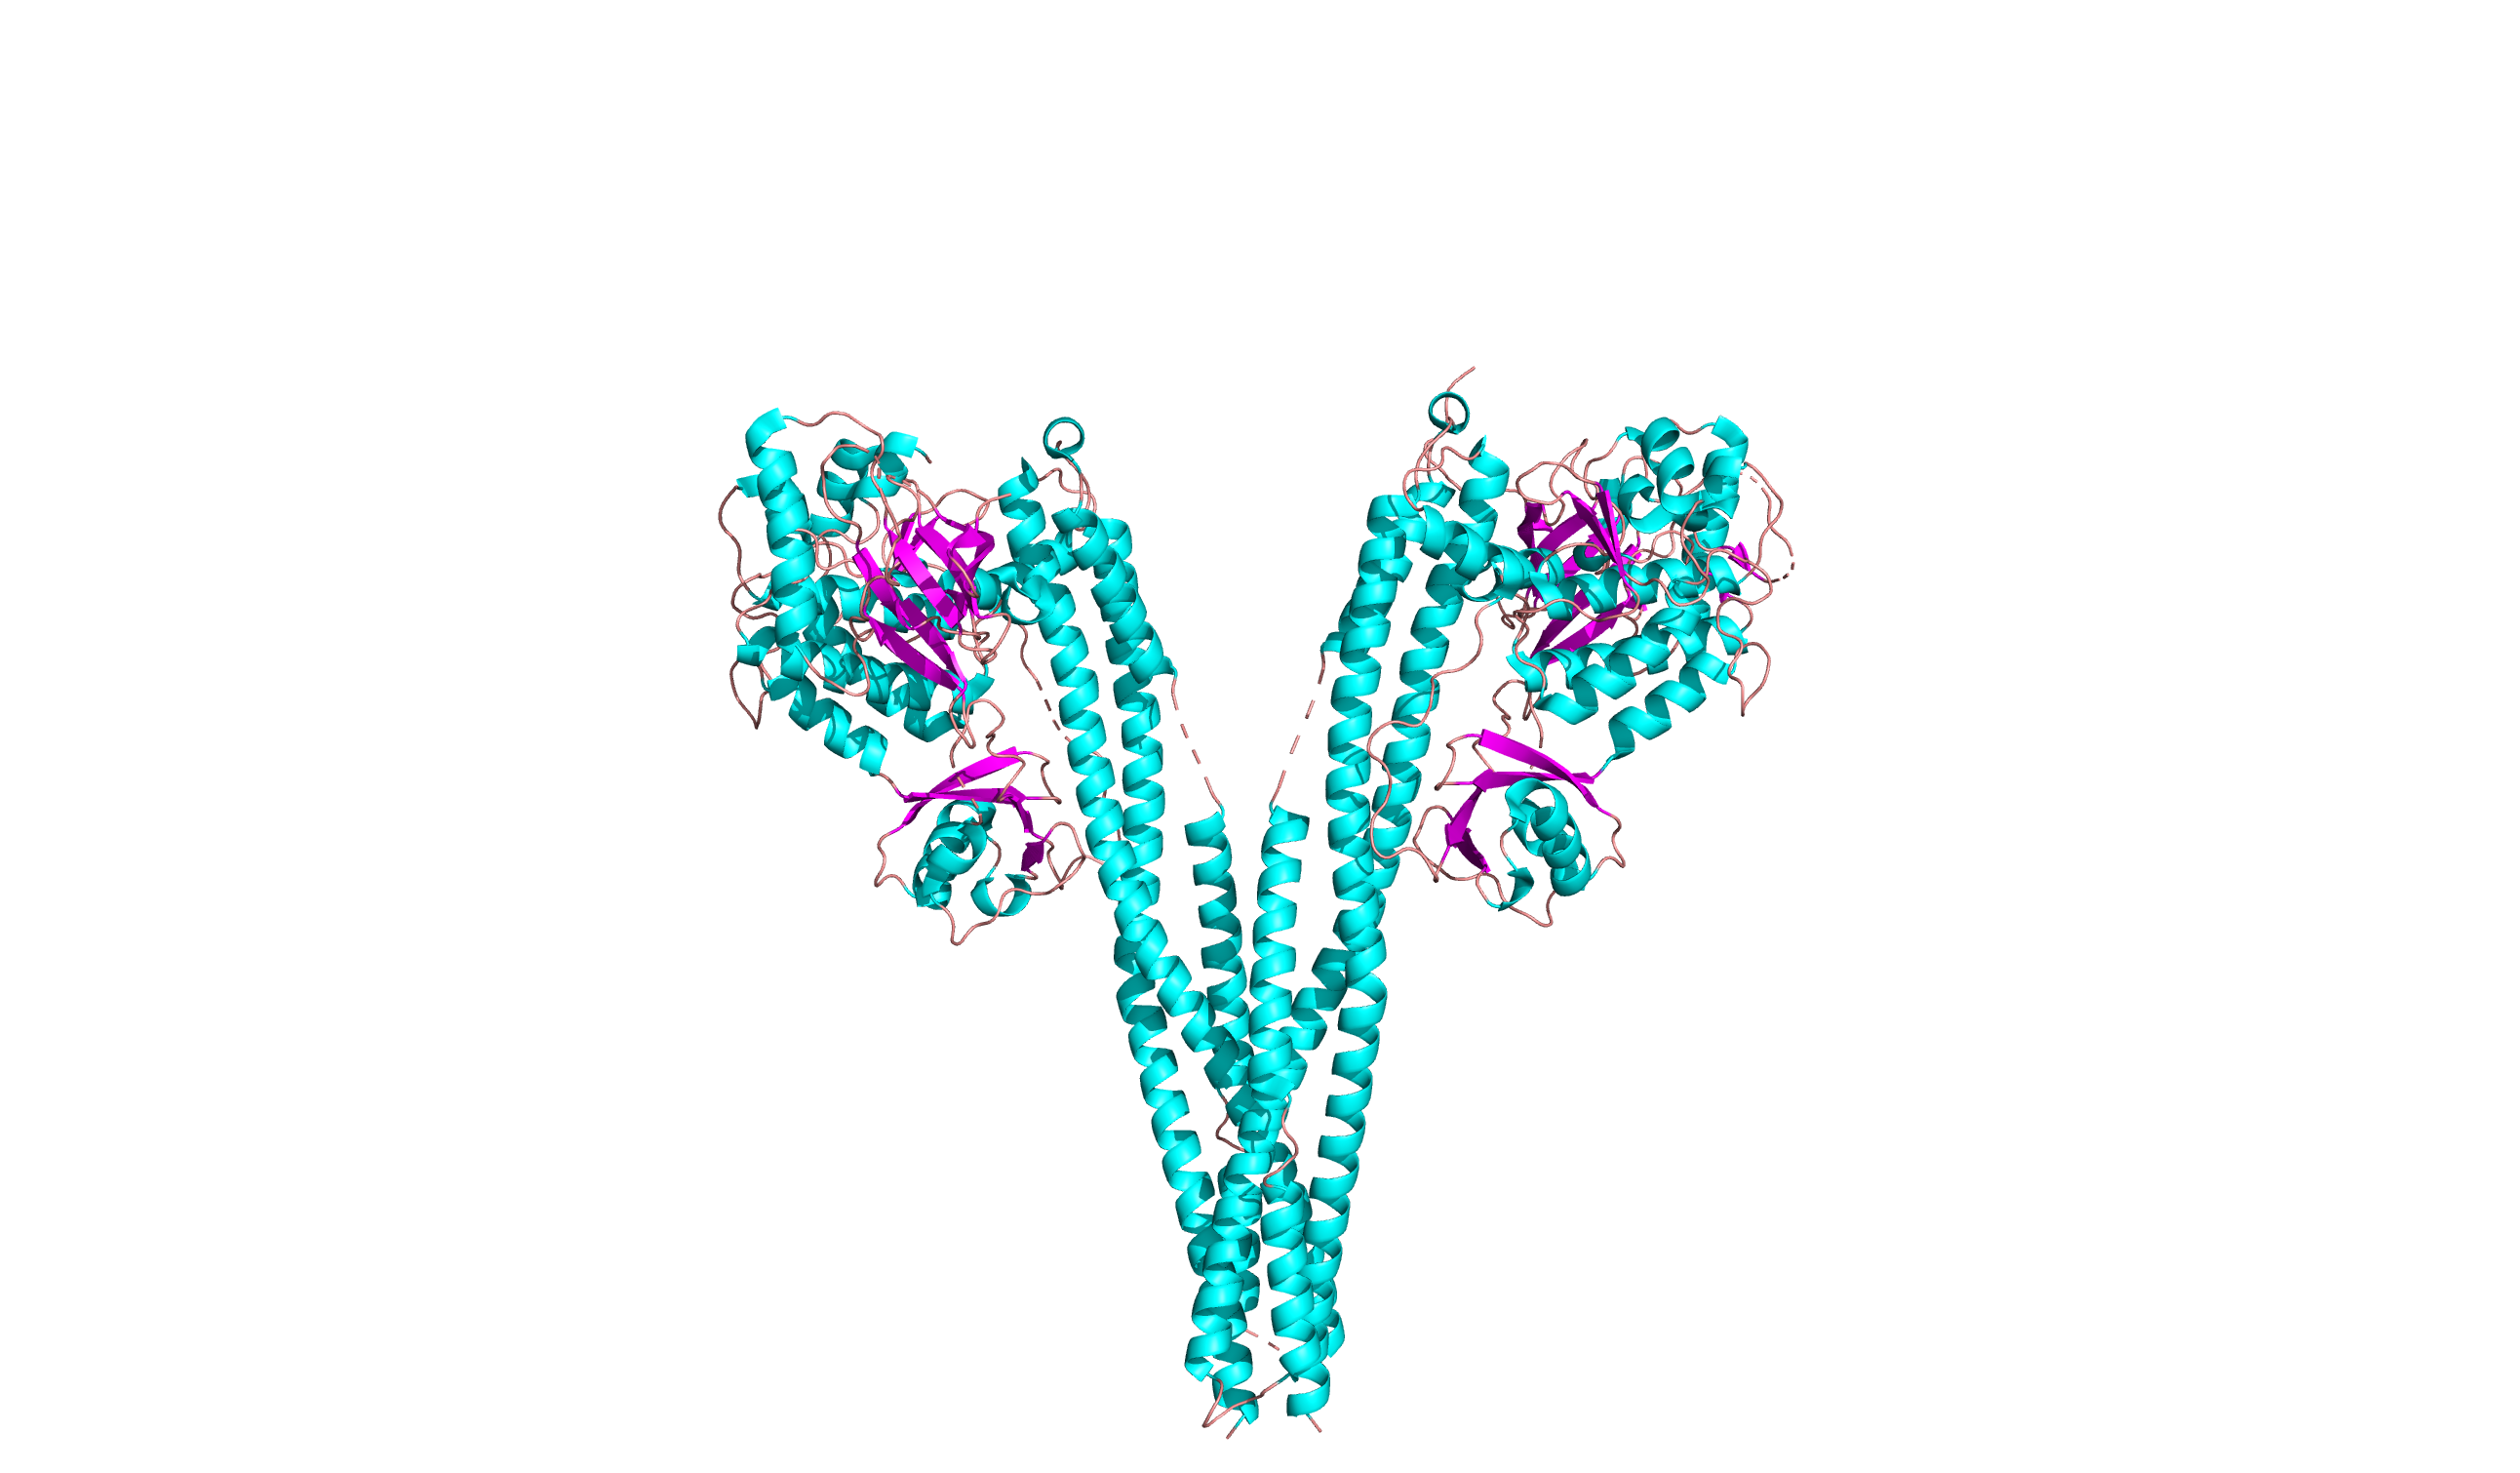
\includegraphics[width=1\linewidth]{Images/4kik_ss.png}
        \caption{X-ray crystallographic structure of IKK-$\beta$}
        \label{fig:4kik}
    \end{figure}

Under normal circumstances, NF-$\kappa$B is sequestered in the cytoplasm through its association with I$\kappa$B proteins, preventing its nuclear localization (Chen et al., 2015). The deficiency of IKK-$\beta$ in adipose cells was shown to prevent the free fatty acid-induced expression of target genes that encode inflammatory mediators (i.e., TNF-$\alpha$ and IL-6) while its activation suppressed the expression of anti-inflammatory cytokines (i.e., leptin and adiponectin) (Jiao et al., 2011). 

This underscores the relevance of the IKK-$\beta$/NF-$\kappa$B pathway to overall IR since the elimination of IKK-$\beta$ and inhibition of NF-$\kappa$B results in improved glucose tolerance and insulin sensitivity (Chen et al., 2015). In instances of insulin resistance, serine phosphorylation of IRS-1 has been correlated with the activation of the IKK-$\beta$ complex (Gao et al., 2002; Liu et al., 2012). Gao et al. (2002) found that serine phosphorylation of IRS-1 at Ser(312) in response to TNF-$\alpha$ was reduced in cells treated with IKK inhibitor 15 deoxy-prostaglandin and in cells from IKK-knockout mice. Thus, IRS-1 is suggested to be a direct substrate of IKK-$\beta$, which results in IRS-1 serine phosphorylation and, ultimately, impairment of the PI3K insulin signal transduction pathway (See \ref{fig:InsulinPath}). Consequently, inhibiting the binding between IRS-1 and IKK-$\beta$ may mitigate insulin resistance initially caused by the early-stage termination of the insulin transduction pathway.


\section{Current Treatments for PCOS Insulin Resistance}

Generally, treatment for PCOS varies due to the heterogeneity of its manifestation. The appropriate treatment depends on the individual’s PCOS phenotype as therapeutics for certain symptoms may exacerbate others. For instance, oral contraceptives are widely used to treat menstrual irregularities and hyperandrogenism. However, triphasic progestin-based oral contraceptives have been seen to worsen insulin resistance. To avoid this, one may opt for norethindrone-only contraceptives as an alternative (Dunaif, 1997).  

Hence, to specifically address insulin resistance, metformin, myo-inositol, and thiazolidinediones have commonly been prescribed as well as the novel berberine supplement isolated from traditional Chinese medicine (See Table \ref{tab:Treatment}). 

% \usepackage{tabularray}
\begin{table} [h]
    \centering
    \caption{PCOS Insulin Resistance Treatment Options}
    \label{tab:Treatment}
\noindent\begin{minipage}{\linewidth}
\resizebox{\linewidth}{!}{%
\begin{tblr}{
  row{1} = {c},
  cell{2}{1} = {r=4}{c},
  cell{2}{2} = {r=4}{c},
  cell{2}{4} = {r=2}{},
  cell{4}{4} = {r=2}{},
  cell{6}{1} = {c},
  cell{6}{2} = {c},
  cell{7}{1} = {r=3}{c},
  cell{7}{2} = {r=3}{c},
  cell{7}{4} = {r=3}{},
  cell{10}{1} = {r=3}{c},
  cell{10}{2} = {r=3}{c},
  cell{10}{4} = {r=3}{},
  hline{1-2,13} = {-}{},
}
\textbf{Treatment} & \textbf{Benefits} & \textbf{Mechanism} & \textbf{Side-Effects~}\\
\textbf{Metformin} & Insulin sensitization & Suppress hepatic glucose synthesis & {Vitamin B12 Deficiency \\(breathlessness, fatigue,  lethargy)}\\
 &  & Improve translocation of GLUT-1 and/or GLUT-4~ & \\
 &  & Activate AMPK to promote glucose uptake~ & Lactic acidosis (severe overdose)\\
 &  & Promote adiponectin in endometrial tissues & \\
\textbf{Myo-inositol} & Insulin sensitization~ & {Activation of PI3K/AKT pathway, activating \\glycogen synthase and GLUT-4 translocation~} & {Nausea, diarrhea, abdominal pain, \\fatigue, headache, dizziness~}\\
\textbf{TZDs} & Insulin sensitization & {Act on PPAR-γ to stimulate insulin activity \\through post-insulin receptor mechanism~} & {Hepatotoxicity: severe reversible liver \\failure, liver injury, and death}\\
 &  & {PTP1B inhibitor to promote tyrosine phosphorylation \\of insulin receptor and IRS-1} & \\
 &  & {IKK-β inhibitors to inhibit serine phosphorylation \\of IRS-1} & \\
\textbf{Berberine}~ & Insulin sensitization & Activate AMPK to promote glucose uptake~ & {Allergic reactions, drug-drug interactions, \\and toxicity consequences (altered liver \\function, gastric issues, hemorrhagic \\inflammation, hepato- and hematotoxicity, \\damage to immune cells)}\\
 &  & {PTP1B inhibitor to promote tyrosine phosphorylation \\of insulin receptor and IRS-1} & \\
 &  & IKK-β inhibitor to inhibit serine phosphorylation of IRS-1 & 
\end{tblr}
}
\end{minipage}
\end{table}

Metformin is the most widespread therapeutic prescribed to those suffering from insulin resistance due to its ability to suppress glucose synthesis in the liver and increase insulin sensitivity via weight loss (Dunaif, 1997). Metformin acts as an insulin sensitizer by improving the translocation of glucose transporters, GLUT-1 and/or GLUT-4 to cell membranes, activating the  5'-adenosine monophosphate-activated protein kinase (AMPK) signaling pathway responsible for promoting glucose uptake, and promotes the use of insulin-sensitizing molecules like adiponectin in endometrial tissues (Zhao et al., 2023). 

Although metformin has its benefits, its long-term use can result in vitamin B12 deficiency. Consequently, B12 supplementation may be necessary to mitigate symptoms of the deficit such as breathlessness, fatigue, and lethargy (NHS, 2022). Furthermore, it may–though rarely–cause metformin-associated lactic acidosis in cases of severe overdose (Dyatlova, 2023).


Similarly, the sugar-alcohol supplement myo-inositol, has been observed to aid in insulin sensitivity (Zhao et al., 2023). After insulin-dependent stimulation and activation of phosphatidyl-inositol-specific phospholipase C, the liver releases inositol phosphoglycans that contain either myo-inositol or d-chiro-inositol which eventually activate glycogen synthase through the PI3K/AKT pathway. Ultimately, this inactivates GSK3, enhances glycogen synthase and GLUT-4 translocation, and glucose uptake (Merviel et al., 2021).  

On the other hand, thiazolidinediones (TZDs) are true insulin sensitizers as they act on the nuclear receptor, peroxisome proliferator-activated receptor gamma (PPAR-$\gamma$), thus enhancing insulin activity through a post-insulin receptor mechanism (Huang et al., 2016; Zhao et al., 2023). Moreover, TZDs are PTP1B inhibitors and irreversible allosteric IKK-$\beta$ inhibitors, thus promoting tyrosine phosphorylation of IR and IRS-1 and inhibiting IRS-1 serine phosphorylation respectively (Verma et al., 2019; Elkamhawy et al., 2020). TZDs thus improve insulin sensitivity without altering body weight and lower steroid hormone levels in both lean and obese women with PCOS. 

However, some TZDs have been identified as hepatotoxic. For instance, troglitazone, the first compound approved by the FDA in the US, was withdrawn due to multiple hepatic failures and deaths reported after use (Scheen, 2001). Additionally, some cases of severe reversible liver failure or liver injury have been reported among patients on rosiglitazone and pioglitazone, two other TZDs with similar blood-glucose control efficacy as troglitazone (Scheen, 2001; National Institute of Diabetes and Digestive and Kidney Diseases, 2018). 

\section{Novel Treatments for PCOS Insulin Resistance}

Due to the downsides of current treatment including their contraindications (i.e., renal impairment, hepatic disease, heart failure, respiratory problems), natural bioactive compounds may be used as alternative treatment as they are relatively less toxic than synthetic drugs. For instance, plant-derived isoquinoline alkaloids like berberine, coptisin, palmatine, epiberberine, and jatrorrhizine have been used in traditional medicine to modulate hyperglycemia and hyperlipidemia (Utami et al., 2023). 

Specifically, berberine is a benzylisoquinoline alkaloid that has been traditionally used in China, India, and the Middle East for centuries for its blood sugar regulation properties and may be isolated from \textit{Berberis}, \textit{Coptis}, \textit{Corydalis}, and \textit{Mahonia}. It has recently been found to “reduce blood glucose, increase insulin secretion, reduce body weight and lipid levels, attenuate glucose tolerance and insulin resistance by activating the AMPK pathway, increase glucagon-like peptide-1 (GLP-1) levels, attenuate reactive oxygen species (ROS) production, reverse mitochondrial dysfunction, and suppress inflammation” (Utami et al., 2023). In a 3-month treatment trial for patients with type 2 Diabetes, berberine performed just as well as metformin in lowering patient fasting and prandial blood sugar and insulin in addition to decreasing triglycerides, total cholesterol, and low-density lipoprotein cholesterol. Additionally, no liver or kidney damage was observed in any of the research participants (Yin et al., 2008).

Berberine improves insulin sensitivity via the AMPK pathway which increases AKT phosphorylation, opposing the disruption of the AKT/PI3K/IRS-1 signaling pathway in the insulin-resistant state, such that the expression and translocation of GLUT-4 is stimulated such that glucose uptake by the cell is increased (Utami et al., 2023). Furthermore, berberine inhibits the catalytic activity of PTP1B such that the tyrosine phosphorylation of insulin receptor and IRS-1 is enhanced (Zhang et al., 2021), and it also inhibits IKK-$\beta$ activity by modifying Cys179 and suppressing the phosphorylation of IKK-$\beta$ at Ser181 (Pandey et al., 2008; Utami et al., 2023). In a study of rats with gestational diabetes mellitus, berberine binding to IKK-$\beta$ reduced insulin resistance (Li et al., 2022). Thus, due to the synergistic modulation of different signaling pathways (i.e.,IKK/NF-$\kappa$B and IRS-1/AKT), berberine and similarly structured alkaloids are potential natural therapeutic options that may exhibit equal or greater efficacy.

Moreover, berberine has not been linked to elevating serum enzymes nor has it been observed to damage cells as measured by LDH production (Grout, 2019; National Institute of Diabetes and Digestive and Kidney Diseases, 2020). Additionally, it does not cause lactic acidosis or vitamin B12 deficiency like metformin, and it does not run the risk of excessive lowering of blood sugar. Furthermore, as berberine lowers homocysteine levels, thus improving heart function in those with congestive heart failure relative to placebo (Chang et al., 2012; Wright, 2017), it may be used for individuals with certain cardiovascular abnormalities that may not receive other drugs due to contraindications.  

Nevertheless, some allergic reactions may arise, such as rashes, itching, swelling, dizziness, or difficulty in breathing. Drug-drug interactions may occur with other medications digested in the liver such as those addressing blood pressure, cholesterol, mental health disorders, seizures, organ transplants, and autoimmune diseases (Moniuszko, 2023). It has been reported that the toxicity of pure berberine compounds is much greater than the toxicity of plant extract fractions, where sub-acute concentrations may lead to adverse effects (e.g.,  altered liver function, gastric troubles, hepato- and hematotoxicity, hemorrhagic inflammatory consequences, damage to immune cells and induced apoptosis) (Singh \& Sharma, 2018). However, a recent study has determined a safe dose of berberine for humans to avoid detrimental effects (2.97g/kg body weight) as well as forms that may improve its toxicity value and bioavailability (i.e., berberine hydrochloride) (Utami et al., 2023). Therefore, considering the advantages and disadvantages of berberine as treatment for insulin resistance in women diagnosed with PCOS, it would be beneficial to structurally modify berberine to enhance its insulin sensitization effects while simultaneously reducing its toxicity, and investigate whether or not a similar compound may be sourced from plants or other living organisms. 
